% The design section should give an overview of the theoretical system design
% It should also disclose the development tools used
\clearpage
\section{Design}

The system is required to integrate with two existing vehicle architectures. In the first configuration,
the vehicle is powered by a hydrogen cell kit shown on figure~\ref{fig:protium}. This kit uses an existing
controller that is operated over \verb|UART|, by a custom PCB called the \textbf{Master Controller}, as shown on figure~\ref{fig:network_master}.
In the second configuration, the fuel cell is managed directly by a custom-designed board referred to as the
\verb|Fuel Cell Control Unit (FCCU)|, as shown on figure~\ref{fig:network_fccu}. The telemetry system must be compatible with both setups.

\begin{figure}[!htb]
    \centering
    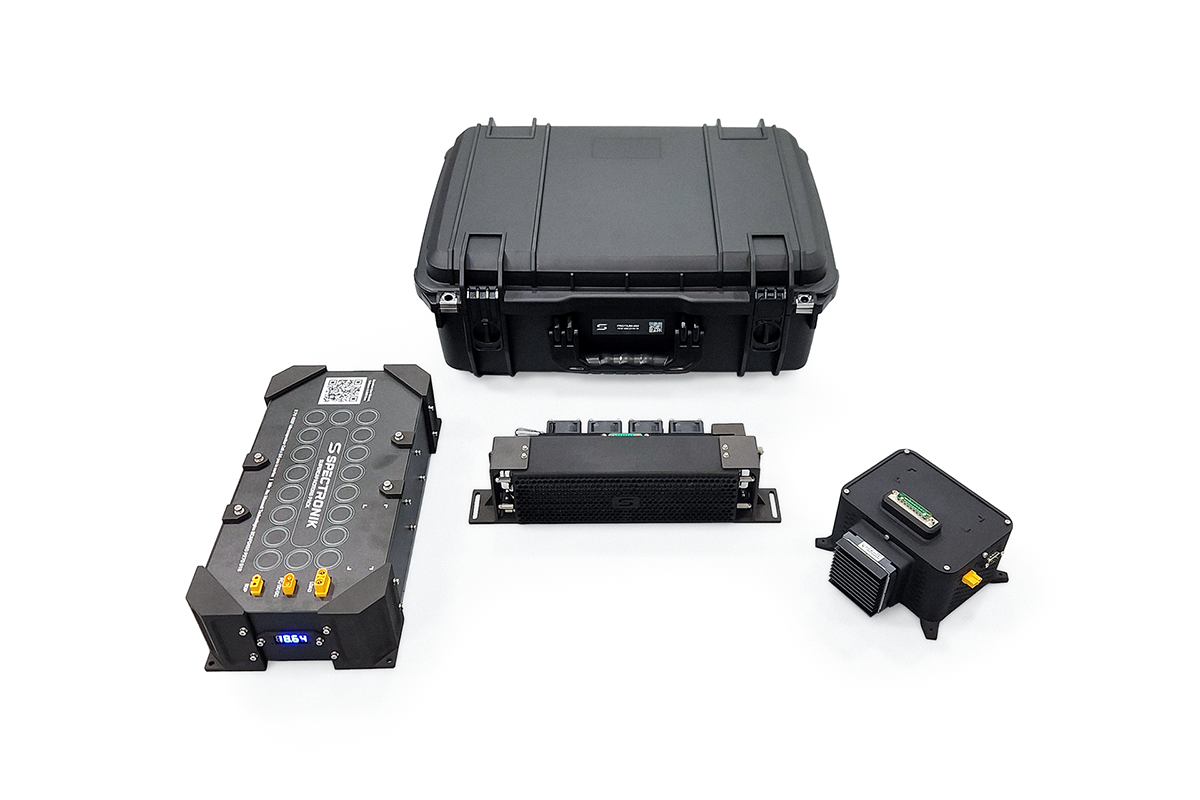
\includegraphics[width=\textwidth]{images/hardware/protium.png}\par
    \caption{Protium hydrogen cell kit}
    \label{fig:protium}
\end{figure}

In addition to interfacing with the vehicle's powertrain components, the system must also integrate with a steering
wheel PCB responsible for capturing driver inputs. This communication must be done over the \verb|Control Area Network (CAN)|
protocol. This PCB includes a button that the driver presses to indicate the completion of a lap. This information is critical during
the race, as teams are required to complete a fixed number of laps and are responsible for tracking lap completion independently.

\begin{figure}[!htb]
    \centering
    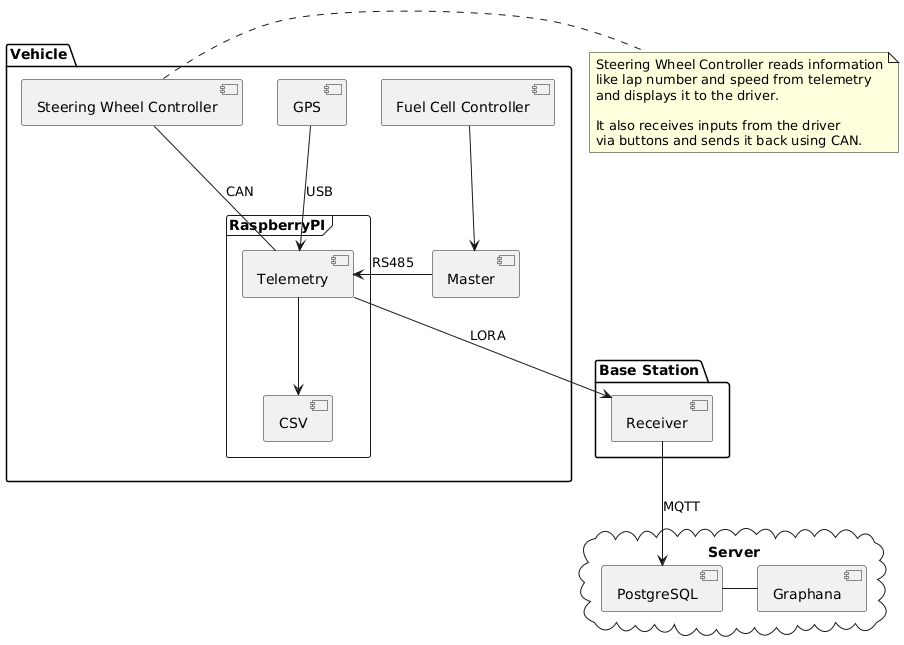
\includegraphics[width=0.8\textwidth]{images/diagrams/network_master.png}\par
    \caption{Vehicle communication when using Protium Kit}
    \label{fig:network_master}
\end{figure}

\begin{figure}[!htb]
    \centering
    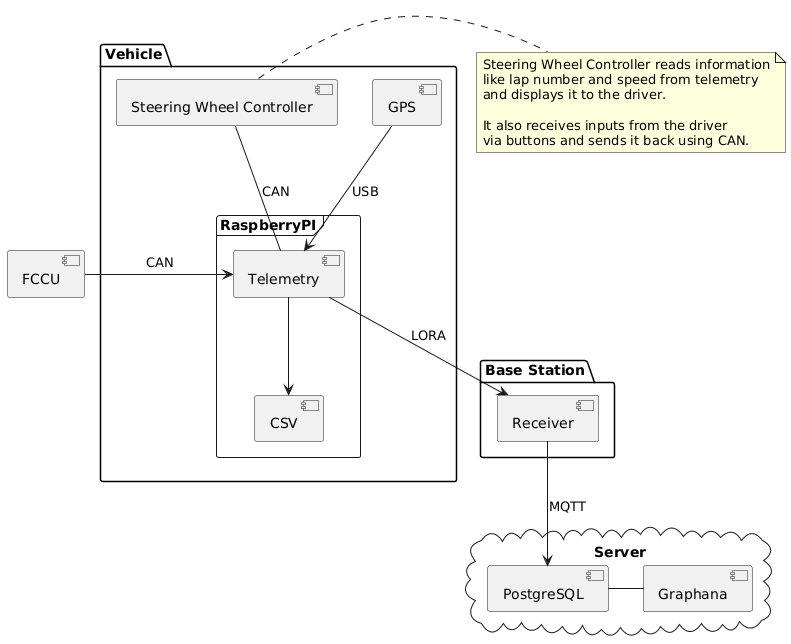
\includegraphics[width=0.8\textwidth]{images/diagrams/network_fccu.png}\par
    \caption{Vehicle communication when using FCCU}
    \label{fig:network_fccu}
\end{figure}
\FloatBarrier

\clearpage
\subsection{Reasoning behind using Linux}
At first glance, using a Linux-based system for a race telemetry application may appear excessive.
However Linux offers several advantages that make it well suited for this type of application when
compared to a bare-metal approach.

One key benefit of using Linux is the availability of a filesystem and a user-space environment, which
significantly simplifies application development and debugging. Access to standard tools, logs and familiar
development workflows reduces development time and improves maintainability.

Another important advantage is Linux's extensive support for a wide range of hardware.
Many communication interfaces and peripherals are supported directly by the kernel or through
mature drivers, allowing development efforts to focus on high-level application login rather than
low-level protocol implementation~\cite{jay-carlson-embedded-linux}.

Finally, running on Linux enables future system expansion beyond basic telemetry functionality. In particular,
it allows for the potential integration of more advanced applications, such as autonomous driving,
which would be impractical or impossible to implement on a traditional bare-metal embedded system.

\subsection{Distributions}

After selecting Linux as the base operating system, the next step was to examine Linux distributions
suitable for embedded systems. The evaluation focused on factors such as system size, stability,
ease of customization and suitability for deployment on resource-constrained hardware.

\paragraph{Debian}
\verb|Debian| is widely regarded as a stable and secure Linux distribution. It serves as the
foundation for many other distributions, including \verb|Ubuntu| and \verb|Tails|~\cite{reasons-to-use-debian}.
Debian provides a large collection of prebuilt packages and extensive documentation.
However, as a general-purpose distribution, it typically includes many components
that are not required in embedded applications, which can lead to increased system size.

\paragraph{Rasperry Pi OS}
\verb|Raspberry Pi OS| is a Debian-based distribution designed primarily for educational and
general-purpose use. It offers good hardware support for a wide range of peripherals and is commonly
used during early development and prototyping. Its default configuration includes a number
of user-facing tools and graphical components that are often unnecessary for dedicated embedded systems.

\paragraph{DietPI}
\verb|DietPI| is a minimal Debian-based distribution designed to achieve a very small system footprint.
Its lightweight nature makes it suitable for resource-constrained environments.
However, the minimal default configuration often requires significant manual setup, which
can increase development effort and reduce maintainability in more complex projects.

\paragraph{Ubuntu Core}
\verb|Ubuntu Core| is an embedded-focused variant of Ubuntu that emphasizes reliability through an immutable
system design. Applications and services are delivered in the form of \verb|snap| packages, which simplifies
dependency management and improves isolation~\cite{ubuntu-core-manual}.
While this approach enhances robustness, it also increases storage requirements due to package duplication,
which may be a limitation in sme embedded systems.

\paragraph{OpenWrt}
\verb|OpenWrt| is an open source Linux distribution originally deigned for networking devices.
It is optimized for small system size, security and network use cases~\cite{openwrt-manual}.
Although well suited for routers and network appliances, its specialized focus can limit flexibility
when used as a general-purpose embedded platform.

None of the evaluated distributions fully satisfied the requirements of flexibility,
customization and long-term maintainability, which motivated the use of a custom-built Linux distribution.

\subsection{Creating custom distributions}

To achieve greater control over the system configuration and hardware support, this project uses
a custom Linux distribution. Several approaches to building such distributions were considered
and evaluated based on their complexity, flexibility and sustainability for embedded development.

\paragraph{From scratch}
Building a Linux distribution entirely from scratch is one possible approach.
It provides control over every component of the system and offers valuable insight into the internal
mechanisms of the Linux operating system~\cite{linux-from-scratch}. However, this level of control
was not required for the scope of this project. Developing a system from scratch would introduce
significant complexity and increase development time without providing corresponding benefits.

\paragraph{Buildroot}
\verb|Buildroot| is a popular tool for generating custom embedded Linux systems and is often considered
one of the simplest solutions available. It provides a centralized configuration file
that allows the developer to select system features and packages, while the build process is managed through \verb|Makefiles|.
Each package is defined by a \verb|.mk| file that specifies how it is downloaded, configured,
compiled and installed.

While this approach simplifies initial setup, Buildroot offers limited build caching, which results in
unnecessary rebuilds during development. Additionally, the configuration structure is
inherently unordered, making large configurations harder to maintain. The available
documentation, although comprehensive, is difficult to navigate due to its structure and presentation,
which further reduces development efficiency~\cite{buildroot-manual}.

\paragraph{Yocto}
\verb|Yocto| is an open-source framework for building custom Linux-based systems, specifically designed for
embedded applications. It provides a high level of abstracton through the use of \verb|recipes|,
which define how individual components, packages or features are built and how they are integrated
into the final system. These recipes can be reused and layered, allowing for scalable and maintainable
system configurations.

Although Yocto introduces additional complexity compared to simpler tools such as \verb|Buildroot|,
it offers significantly better documentation and a large, active community.
These factors improve long-term maintainability and reduce development time, making Yocto
well suited for projects that require flexibility, extensibility and control over the final system image~\cite{yocto-manual}.\\

Based on this evaluation, Yocto was selected as the most suitable solution for building the base system used in the project.
\input{design/hardware/main_board}
\clearpage
\input{design/hardware/modules}
\clearpage
\subsection{Development Tools}
In Embedded linux development it is common to use any text editor with code syntax highlighting.
This project uses \verb|VSCode| as its development platform.

For compiling the \verb|C++| code it uses \verb|CMake| with the following \verb|CMakeLists.txt| file.

\begin{figure}[!htb]
    \centering
    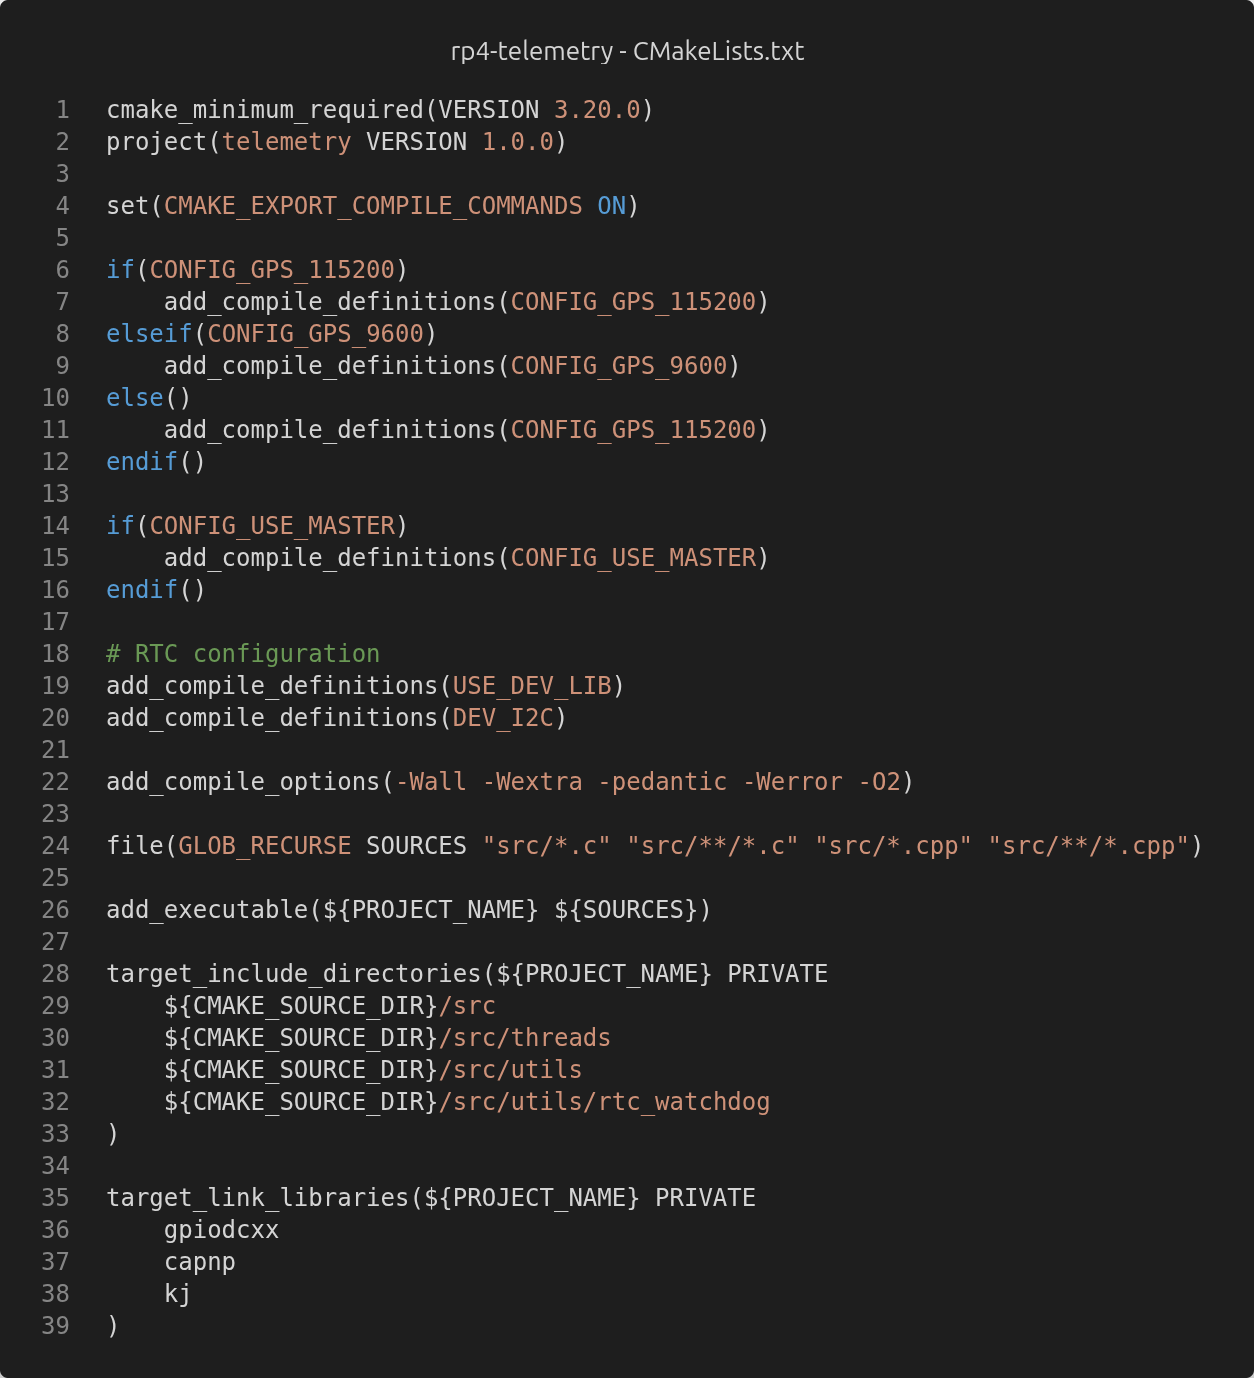
\includegraphics[width=\textwidth]{images/code/cmake.png}\par
    \caption{Binding the CAN socket}
    \label{fig:code-cmake}
\end{figure}
\FloatBarrier

In that file first the preprocessor directives used in code are set.
After that compile rules are made stricter for ensuring good practices.
Lastly all of the code and header files are added and used libraries are linked.